\documentclass[xcolor={dvipsnames}]{beamer}

\usepackage{lmodern}
\usepackage[utf8]{inputenc}
\usepackage{amssymb, amsmath, amsthm, graphicx}
\usepackage[super]{nth}
\usepackage{tikz}

\usetheme{Frankfurt}
\renewcommand{\phi}{\varphi}
\renewcommand{\epsilon}{\varepsilon}
\newcommand{\df}[1]{\textcolor{BrickRed}{\emph{#1}}}
\renewcommand{\th}[1]{\textcolor{Fuchsia}{\emph{#1}}}
\renewcommand{\hat}{\widehat}

\newcommand{\cD}{\mathcal{D}}
\newcommand{\cL}{\mathcal{L}}
\newcommand{\cM}{\mathcal{M}}
\newcommand{\cN}{\mathcal{N}}
\newcommand{\cX}{\mathcal{X}}
\newcommand{\cZ}{\mathcal{Z}}
\newcommand{\EE}{\mathbb{E}}

\newcommand{\RR}{\mathbb{R}}

\DeclareMathOperator*{\argmin}{argmin}
\DeclareMathOperator{\Var}{Var}
\DeclareMathOperator{\MSE}{MSE}
\DeclareMathOperator{\Bernoulli}{Bernoulli}

\title[DATA 607]{DATA 607 Statistical and Machine Learning\\
Session 1}
\author{Matthew Greenberg}
\institute[]{Department of Mathematics and Statistics\\
University of Calgary}
\date{Session 1 --- 24.02.2020}

\begin{document}

\frame{\titlepage}

\begin{frame}
    \frametitle{This Evening's Agenda}
    \tableofcontents
    \end{frame}

% \begin{frame}
%     \frametitle{This Evening's Agenda}

%     \begin{enumerate}
%         \setlength\itemsep{1em}
%         \item Course information

%         % \medskip
%         % \begin{itemize}
%         %     \setlength\itemsep{0.5em}
%         %     \item goals, non-goals
%         %     \item logistics
%         %     \item topics, tentative schedule
%         % \end{itemize}
        
%         \item Big picture
        
%         \item Models
        
%         \item Nonparametric models for regression and classification
        
%         % \medskip
%         % \begin{itemize}
%         %     \setlength\itemsep{0.5em}
%         %     \item What are statistical learning and machine learning?
%         %     \item How do they fit into data science?
%         %     \item What kinds of machine learning are there?
%         %     \item How does machine learning relate to/differ from \underline{\hspace{1cm}}?
%         % \end{itemize}
%     \end{enumerate}
% \end{frame}
% 
% \begin{frame}
    % \begin{enumerate}\setcounter{enumi}2
%         
%     
% 
%         \item Models
%         \begin{itemize}
%             \item Dichotomies 
%             \setlength\itemsep{0.5em}
%             \item \begin{itemize}
%                 \item Supervised/unsupervised
%                 \item Parametric/nonparametric
%                 \item Discriminative/generative
%             \end{itemize}
%             \item Characteristics
%             \begin{itemize}
%                 \item complexity
%                 \item bias
%                 \item variance
%             \end{itemize}
%             \item Prediction, generalization
%             \item Training, testing
%             \item Model selection and evaluation
%         \end{itemize}
%     \end{enumerate}
%     
% 
% \end{frame}

\section{Course Information}

\begin{frame}
    \frametitle{Course Information}

    \begin{itemize}
        \setlength\parskip{0.75em}
        \item \textbf{Instuctor:} Matthew Greenberg
        
        \textbf{Email:} \texttt{mgreenbe@ucalgary.ca}

        \textbf{Office hours:} Mondays and Wednesdays, 16:00-17:00

        \item \textbf{TA:} Mingchen Ren
        
        \textbf{Email:} \texttt{ming.ren@ucalgary.ca}
        
        \textbf{Office hours:} TBA

        \item \textbf{Textbook:} Aur\'elien Geron, \emph{Hands on Machine Learning with Scikit-Learn and Tensorflow, \nth{2} Edition}, O'Reilly.
        
        \textbf{Also useful:} James et al., \emph{An introduction to Statistical Learning (with Applications in R)}, Springer, \th{\textsc{Free Online}}.
    \end{itemize}
\end{frame}

\begin{frame}

    \begin{itemize}
        \setlength\parskip{1em}
        \item \textbf{Evaluation:} 5 homework assignments, equally weighted
        
        \textbf{Due dates:} 04.03, 11.03, 18.03, 25.03, 01.04 at 23:59

        \textbf{Distribution:} $\sim$1 week before due date

        \textbf{Submission:} Jupyter notebook format (\texttt{.ipynb}), via D2L

        \textbf{Conversion:} Minimum \% required for...

        \begin{center}
        \begin{tabular}{c|c|c|c|c|c|c|c|c|c|c}
            A$+$&A&A$-$&B$+$&B&B$-$&C$+$&C&C$-$&D$+$&D\\\hline
            95&90&85&80&75&70&65&60&55&50&45
        \end{tabular}
    \end{center}
    \end{itemize}
\end{frame}

\begin{frame}
    \begin{itemize}
        \setlength\parskip{1em}
        \item \textbf{Description:} From the calendar:

        \bigskip
        \begin{quote}
        Advancement of the linear statistical model including introduction to data
        transformation methods, classification, model assessment and selection.
        Exposure to both supervised learning and unsupervised learning.
    \end{quote}

    \item \textbf{Topics}
    \begin{enumerate}
        \setlength\parskip{0.5em}
        \item Introduction: Models (1 session)
        \item Nonparametric models for supervised learning (3 sessions)
        \item Deep models for supervised learning (4 sessions)
        \item Unsupervised and self-supervised learning (4 sessions)
    \end{enumerate}
\end{itemize}
\end{frame}

\begin{frame}
    \frametitle{}

    \begin{itemize}
        \setlength\parskip{1em}
        \item \textbf{Software:}
        \begin{itemize}
            \setlength\parskip{1em}
            \item Python: numpy, pandas, matplotlib, scikit-learn, ntlk, tensorflow
            
            \emph{Please ensure you have the latest stable versions of Python 3 and of the a libraries intalled (e.g., via the Anaconda platform).}
            \item Jupyter notebooks: localhost, Google Colab
            
            \emph{Please ensure you have the latest stable version of Jupyter Noteboook/JupyterLab intalled.}
            
            \item Other: Git, markdown, \LaTeX
        \end{itemize}
    \end{itemize}
\end{frame}

\section{Big Picture}

\begin{frame}
    \frametitle{Big Picture}
    \setlength\parskip{1em}


    \textbf{``Definitions''}

    \begin{itemize}
        \setlength\parskip{1em}
        \item \textbf{\textit{Machine learning:}} Using algorithms to learn from data.
        
        \item \textbf{\textit{Algorithm:}} A sequence of explicit instructions for performing a computation.
        
        \item \textbf{\textit{Learn:}} Improve a performance metric. Solve a problem.
        
        \item \textbf{\textit{Data:}} Information. Input to an algorithm.
    \end{itemize}
\end{frame}

\begin{frame}
    \setlength\parskip{1em}
    \frametitle{Jargon}

    What's the difference?
    \begin{itemize}
        \item Data science
        \item Machine learning
        \item Artificial intelligence
        \item Statistical learning
        \item Statistics
    \end{itemize}

    An answer to this question would require precise, broadly accepted definitions of these terms.
    
    These terms suggest different points of view on similar problems and subject matter.
    
    

    

\end{frame}

\begin{frame}
    \setlength\parskip{1em}
    My point of view:
    
    \begin{itemize}
        \setlength\parskip{1em}
        \item \emph{Data science} is characterized by its breadth and inclusivity.
        Exploratory analysis, visualization, and communication are core components.
        \item \emph{Machine learning} and \emph{artificial intelligence} emphasize algorithms, computation, and scale. Prediction and generalization are key performance metrics.
        [This course]
        \item \emph{Statistical learning} emphasizes theoretical guarantees regarding consistency, rates of connvergence, etc.
        \item \emph{Statistics} emphasizes sampling, experimental design, inference, confidence intervals, hypothesis tests, $p$-values\ldots
    \end{itemize}
\end{frame}

\section[Models]{Models}

\begin{frame}
    \setlength\parskip{1em}
    \frametitle{Models}

    A \emph{model} is a structure or a family of structures ostensibly\footnote{apparently or purportedly, but perhaps not actually (from \texttt{lexico.com})} describing a data set.

    A \emph{statistical model} is a model in which this family of structures consists of \emph{probability distributions}.

    The failure of a family member to reflect the structure of data set is measured by a \emph{loss function}.

    \emph{Fitting a model} is the process of determining which member of this family best describes the data set, i.e., minimizes the loss function.

    Some models, after having been fit, can be used for \emph{prediction}.
\end{frame}


% \begin{frame}
% \frametitle{The Simple Linear Regression Model}
% \setlength\parskip{1em}
% The \emph{simple linear regression model} is the family of linear functions
% \[
%    y = \beta_0 + \beta_1 x,\qquad\beta_0,\beta_1\in\RR.
% \]

% \begin{itemize}
%     \item \textbf{Loss function:}
%     The loss function most commonly used for measuring the failure of this model to reflect the
%     structure of a data set $$\cD=\left\{(x_1,y_1),\ldots,(x_n,y_n)\right\}$$ is \emph{mean squared error (MSE)}:
%     \[
%     \MSE(\beta_0,\beta_1,\cD) = \frac1n\sum_{i=1}^n(\beta_0 + \beta_1x_i - y_i)^2
%     \]
% \end{itemize}
% \end{frame}

% \begin{frame}

% \begin{itemize}
%     \setlength\parskip{1em}
%     \item Fitting the simple linear regression model to $\cD$ means finding the values,
%     $\hat\beta_0$ and $\hat\beta_1$, of the parameters  that minimize $\MSE(\beta_0,\beta_1,\cD)$.
%     In symbols,
%     \[
%         (\hat{\beta}_0,\hat{\beta}_1) = \argmin_{(\beta_0,\beta_1)}\MSE(\beta_0,\beta_1,\cD).
%     \]

%     \item Simple linear regression is a \emph{predictive model}.
%     Given a new $x$-value, $x_0$, our model that predicts the corresponding $y$-value to be
%     $$\hat y_0=\hat\beta_0 + \hat\beta_1x_0.$$
%     To quantify our uncertainty this prediction, we need information about the
%     distribution from which $\cD$ was drawn.
% \end{itemize}
% \end{frame}

% \begin{frame}
%     \setlength\parskip{1em}
%     \frametitle{A statistical model for simple linear regression}

%     Suppose we know that $y_i$ was drawn from
%     $\cN(\beta_0 + \beta_1 x_i, \sigma^2)$ for $i=1,\ldots,n$.


%     Let $(x_0,Y_0)$ be a new data point with $Y_0\sim \cN(\beta_0 + \beta_1 x_0, \sigma^2)$.
%     Our predicted value for $Y_0$ is $\hat\beta_0 + \hat\beta_1x_0$.
    
%     Under the above model, the expected squared error in this prediction is
%     \[
%         \EE[(\hat{\beta}_0 + \hat{\beta}_1 x_0 - Y_0)^2] = \left(1 + \frac1n + \frac{(x_0-\bar x)^2}{S_{xx}}\right)\sigma^2.
%     \]
    

% \end{frame}
    
    
        




% \section[Nonparametric Methods]{Nonparametric Methods for Regression and Classification}

% \begin{frame}
%     \frametitle{Nonparametric Methods for Regression and Classification}

    

% \end{frame}


\begin{frame}
    \frametitle{Parametric and Nonparametric Models}
    \setlength\parskip{0.75em}

    \textbf{Parameters} are quantities associated to a model that must be learned from data.

    \textbf{Parametric model:} The number of parameters is independent of the size of the data set.
    \begin{itemize}
        \item Example: The family of Gaussian distributions $N(\mu,\sigma)$ with densities
        \[
            p(x|\mu,\sigma) = \frac1{\sqrt{2\pi}\sigma}e^{-(x-\mu)/2\sigma^2}.
        \]
        \item Example: The simple linear regression model:
        \[
            y=\beta_0 + \beta_1x + \epsilon,\qquad \epsilon\sim N(0,\sigma^2)
        \]
    \end{itemize}
\end{frame} 

\begin{frame}
    \setlength\parskip{0.75em}
    \textbf{Nonparametric model:} The number of parameters depends on the size of the data set.
    \begin{itemize}
        \item Example: Histogram density estimators:
        \[
            p(x|c_1,\ldots,c_n, n) = \text{$c_i$ if $x$ is in bin $i$}
        \]
        \begin{center}
        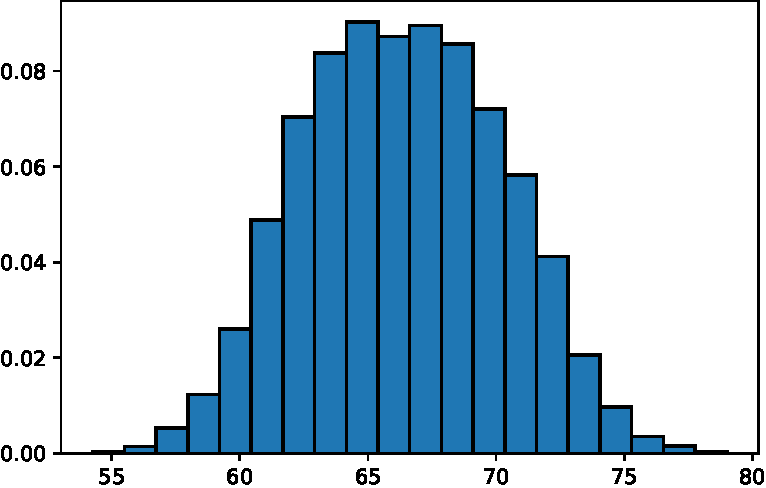
\includegraphics[scale=0.5]{hist.pdf}
        \end{center}
        Typically, we use larger $n$ for larger data sets.
    \end{itemize}
\end{frame}

\begin{frame}
    \frametitle{Generative and Discrimintive Models}
    \setlength\parskip{0.75em}
    \textbf{Generative model:} A model of the distribution from which your data set was drawn.
    \begin{itemize}
        \item Example: Bayes classifier
        \[
            p(x,z) = p(x|z)p(z)
        \]
        \item Mixture of Gaussians
        \[
            p(x) = \sum_i \pi_i p(x|\mu_i,\sigma_i),\quad \pi_i\geq 0,\quad \sum_i \pi_i=1
        \]
        \begin{center}
            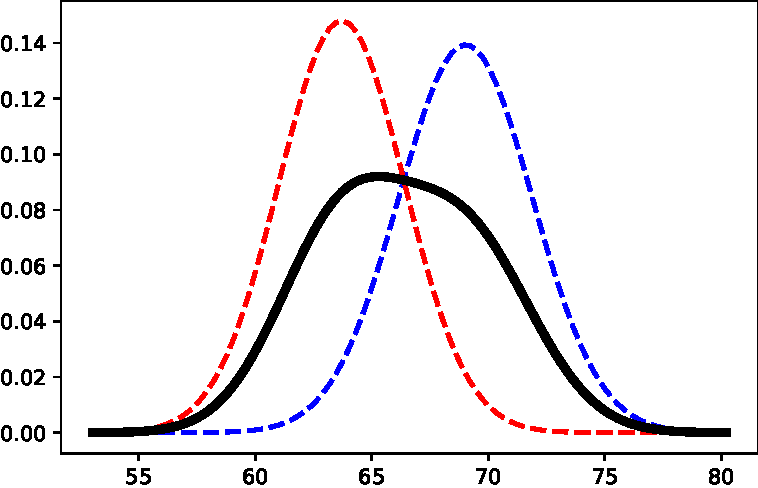
\includegraphics[scale=0.4]{gmm.pdf}
        \end{center}
    \end{itemize}
\end{frame}

\begin{frame}
    \setlength\parskip{0.75em}
    \textbf{Discriminative/Conditional model:} Given a data set consisting of a predictor variable $x$ and
    a response variable $y$, model the conditional distributions $p(y|x)$.
    Most classification and regression models are of this type.
    \begin{itemize}
        \item Example: Simple linear regression
        \[
            y=\beta_0 + \beta_1x + \epsilon,\qquad \epsilon\sim N(0,\sigma^2)
        \]
        \item Example: $k$-nearest neighbor classifier
    \end{itemize}
\end{frame}

\begin{frame}
    \frametitle{Supervised and Unsupervised Learning}
    \setlength\parskip{0.75em}

    \textbf{Supervised learning:} Data is \emph{labelled}.
    \begin{itemize}
        \item Discriminative models
    \end{itemize}

    \textbf{Unsupervised learning:} Data is \emph{unlabelled}.
    \begin{itemize}
        \item Clustering
        \item Mixture models
    \end{itemize}

    Distinction is nebulous in situations where there is no clear notion of label, e.g., density estimation.
\end{frame}
\end{document}